
En una conexión TCP recién establecida (IW = 2 MSS, SSTHRESH = 64 KB) con RTT=200 ms y MSS=2 KB, el host receptor siempre anuncia una AdvertisedWindow de 16 KB. La red está cargada al punto que si una ráfaga fuera de 16 KB o más, se perderían todos los segmentos de la misma.
¿Cuántos rounds se demora en enviar un archivo
de 36 KB?



$$ \mathrm{RTT} = 200 ms $$

$$ \mathrm{MSS} = 2 KB$$

$$ IW = 2 MSS $$

$$ \mathrm{SSTHRESH} = 64 KB $$

$$ \mathrm{rwnd} = 16 KB $$

$$ \mathrm{LimiteDeLaRed} = 16 KB $$

$$ \mathrm{fileSize} = 36 KB $$

Paso los datos a MSS

$$ IW = 2 MSS $$

$$ \mathrm{SSTHRESH} = 32 MSS $$

$$ \mathrm{rwnd} = 8 MSS $$

$$ \mathrm{LimiteDeLaRed} = 8 MSS $$

$$ \mathrm{fileSize} = 18 MSS $$



\begin{figure}[H]
\centering
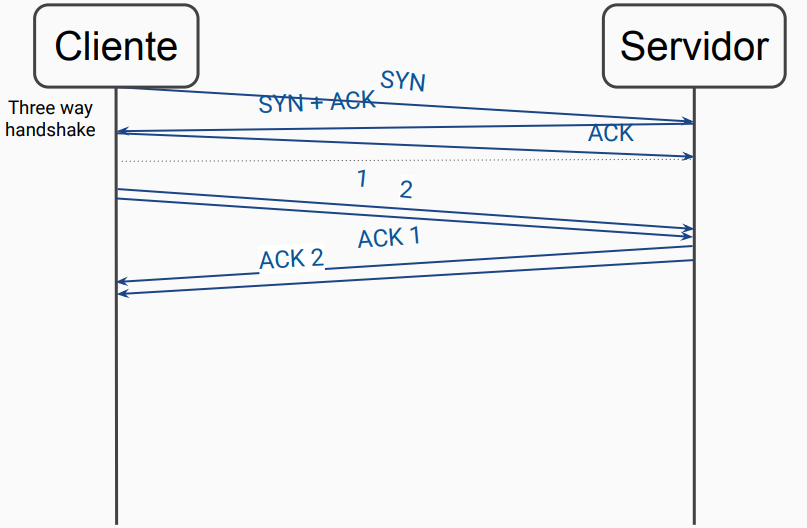
\includegraphics[width=\textwidth]{imagenes/resolucion1.png}
\end{figure}

En una primera instancia se realiza el three way handshake para establecer la conexion TCP. $IW = 2$ entonces $\mathrm{cwnd}_n = 2$. Se envían 2 segmentos, se reciben los 2 ACK correspondientes. Como se está en slow start, $$ \mathrm{cwnd}_{n+1} = \mathrm{cwnd}_n + \#ACK $$

De esta manera, $\mathrm{cwnd}_{n+1} = 2 + 2 = 4 $ y se envían 4 segmentos. De los cuales se reciben los 4 ACKs


\begin{figure}[H]
\centering
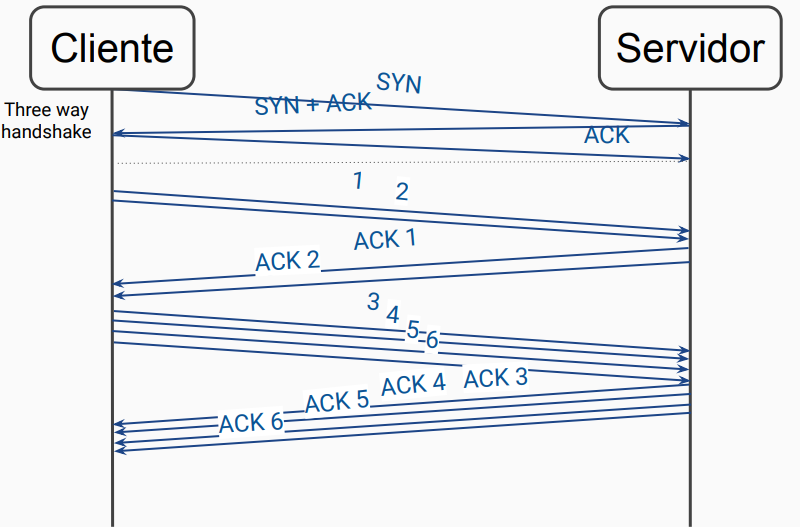
\includegraphics[width=\textwidth]{imagenes/resolucion2.png}
\end{figure}

se sigue en Slow start, por lo que  $\mathrm{cwnd}_{n+2} = \mathrm{cwnd}_{n+1} + \#\mathrm{ACK} = 4 + 4 = 8 $

Se envían entonces los siguientes 8 segmentos, los cuales se pierden ya que $ \mathrm{rwnd} = 8 $

\begin{figure}[H]
\centering
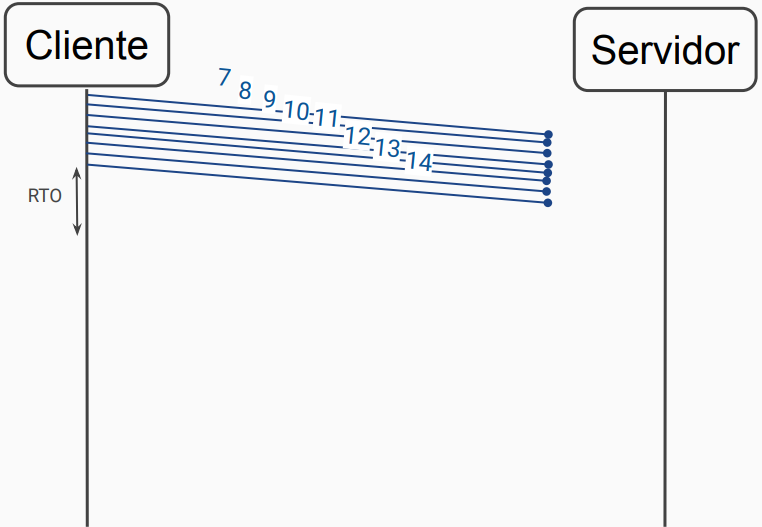
\includegraphics[width=\textwidth]{imagenes/resolucion3.png}
\end{figure}

El cliente se informa de esto por un timeout (RTO). Entonces debe actuarse teniendo en cuenta este evento. El valor de la ventana volverá a ser 1, por lo que $ \mathrm{cwnd}_{n+3} = 1  $. Además se modifica el threshold de acuerdo a $ \mathrm{ssthresh} = \frac{\mathrm{cwnd}_n}{2}  = \frac{8}{2} = 4$.

Se retoma entonces el envío de datos, enviando 1 segmento y recibiendo el ACK correspondiente. Se actualiza la ventana con $\mathrm{cwnd}_{n+4} = 1 +1 = 2$. Se envian entonces 2 y se reciben 2 ACK. Se llega a que $\mathrm{cwnd}_{n+5} = 2 + 2 = 4 $. 

\begin{figure}[H]
\centering
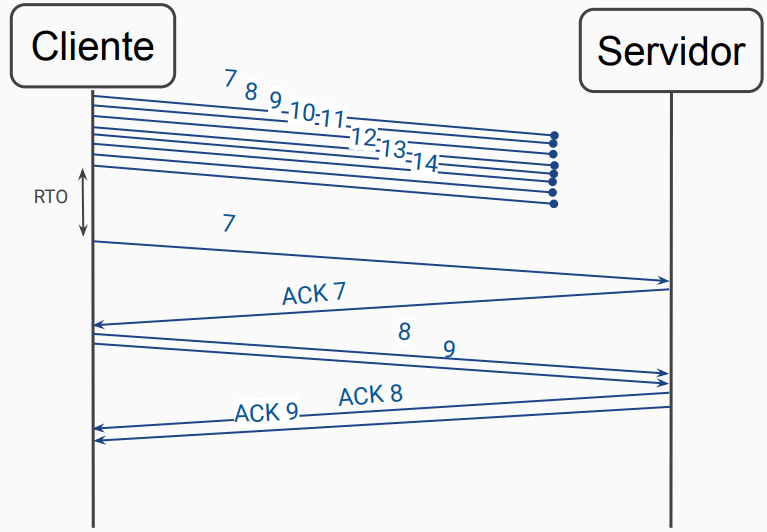
\includegraphics[width=\textwidth]{imagenes/resolucion4.png}
\end{figure}

Recordemos que por el RTO,  $ \mathrm{ssthresh} = 4 $, entonces $\mathrm{cwnd} \geq \mathrm{ssthresh} $. Entonces \textbf{finaliza Slow start y comienza congestion avoidance}.
Continuamos enviando 4 segmentos y recibimos los ACK correspondientes.
Ahora el cálculo de la ventana es distinto

$$ \mathrm{cwnd}_{n+1} = \mathrm{cwnd}_n + \frac{\#\mathrm{ACK}}{\mathrm{cwnd}_n} $$

entonces  $\mathrm{cwnd}_{n+6} = 4 + \frac{4}{4} = 5 $ y se envían 5 segmentos, de los cuales se reciben los 5 ACKs correspondientes. Ya se enviaron 18 MSS y como $\mathrm{fileName} = 18 \mathrm{MSS} $ es el fin de la transmisíon. 

\begin{figure}[H]
\centering
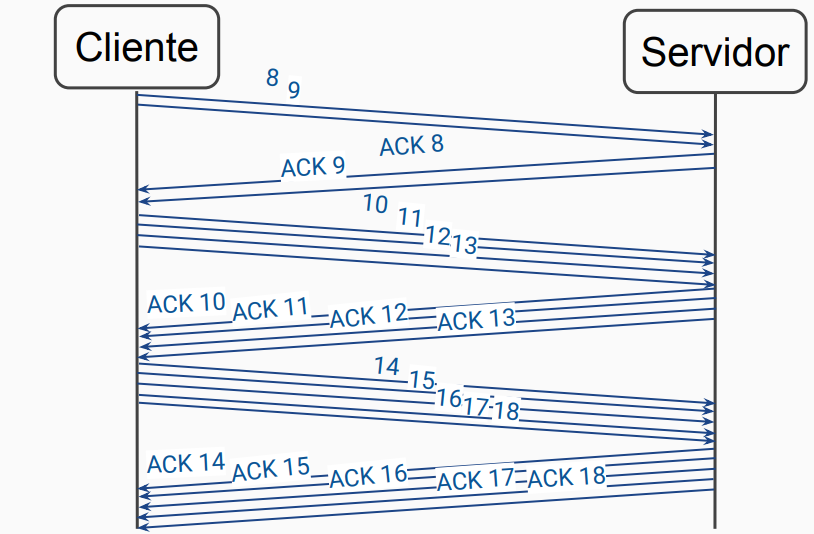
\includegraphics[width=\textwidth]{imagenes/resolucion5.png}
\end{figure}

Lo único que faltaría serian los mensajes correspondientes al cierre, que implica 4 mensajes

\begin{figure}[H]
\centering
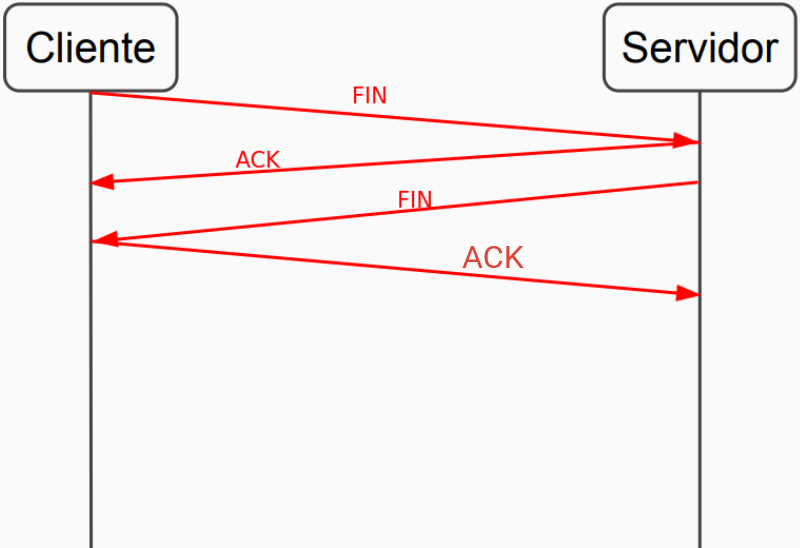
\includegraphics[width=\textwidth]{imagenes/resolucion6.png}
\end{figure}